\documentclass[12pt]{article}

\usepackage{booktabs}% http://ctan.org/pkg/booktabs
\usepackage[utf8]{inputenc}
\usepackage{changepage}
\usepackage{pgfplots}
\usepackage{amssymb}
\usepackage{xcolor}
\usepackage{hyperref}
\usepackage{listings}
\usepackage[T1]{fontenc}
\usepackage[utf8]{inputenc}
\usepackage{adjustbox}
\usepackage{amsmath}
\usepackage{mathtools}
\usepackage{biblatex}

\lstset{
  language=Python,
  numbers=left,
  numberstyle=\tiny,
  stepnumber=1,
  numbersep=5pt,
  tabsize=4,
  basicstyle=\ttfamily,
  columns=fullflexible,
  keepspaces,
}
\hypersetup{
    colorlinks,
    citecolor=black,
    filecolor=black,
    linkcolor=black,
    urlcolor=black
}

% Set page size and margins
% Replace `letterpaper' with `a4paper' for UK/EU standard size
\usepackage[letterpaper,top=2cm,bottom=2cm,left=3cm,right=3cm,marginparwidth=1.75cm]{geometry}

% Useful packages
\usepackage{amsmath}
\usepackage{mathtools}
\usepackage{graphicx}
\newenvironment{para}{\begin{adjustwidth}{13mm}{}}{\end{adjustwidth}}

\newcommand\tab[1][1cm]{\hspace*{#1}}

\newcommand{\tabitem}{\llap{\textbullet}}
\newcommand{\Hsquare}{%
\text{\fboxsep=-.2pt\fbox{\rule{0pt}{1ex}\rule{1ex}{0pt}}}%
}

\newtheorem{Definizione}{Definizione}[subsection]
\newtheorem{Lemma}{Lemma}[subsection]
\newtheorem{Teorema/Definizione}{Teorema/Definizione}[subsection]
\newtheorem{Corollario}{Corollario}[subsection]
\newtheorem{Teorema}{Teorema}[subsection]
\newtheorem{Proposizione}{Proposizione}[subsection]
\newtheorem{Notazione}{Notazione}[subsection]
\newtheorem{Commento}{Commento}[subsection]
\newtheorem{Dimostrazione}{Dimostrazione}[subsection]
\newtheorem{Osservazione}{Osservazione}[subsection]
\newtheorem{Nota}{Nota}[subsection]

\title{Ricerca operativa e pianificazione delle risorse}
\author{spitfire}
\date{A.A. 2023-2024}
\begin{document}
\begin{figure}
    \centering
    
\includegraphics[width=0.35\textwidth]{Images/Logo scienze bicocca.png}
\end{figure}

\vspace{10cm}
\date{A.A. 2024-2025}


\maketitle

\newpage

\tableofcontents
\newpage

\section{Prerequisiti di Algebra Lineare}
\subsection{Matrici e vettori}
Una matrice è una tabella contenente numeri.
Se la tabella è costituita da $m$ righe e $n$ colonne si parla
di una matrice  $m \times n$. 
Una matrice viene detta \textbf{matrice quadrata} se il numero di righe
e colonne coincidono. \newline
Una matrice $1 \times m$ viene detto \textbf{vettore riga m-dimensionale} \newline
Una matrice $m \times 1$ viene detto \textbf{vettore colonna m-dimensionale}. \newline
La notazione maggiormente utilizzata per indicare una matrice è
$$A = [a_{ij}]$$
Con $a_{ij}$ elemento generico della i-esima riga e j-esima colonna della matrice $A$.
Se $A = [a_{ij}]$ è una matrice $m \times n$, la matrice $n \times m$
$$A^T=[a_{ij}]$$
viene detta \textbf{matrice trasposta} della matrice $A$.

Se $A = [a_{ik}]$ è una matrice $m \times p$ e $B = [b_{kj}]$ è una matrice $p \times n$ la loro
\textbf{matrice prodotto} è $m \times n$ e definita come:
$$A \cdot B = C = [c_{ij}] \; con \; c_{ij} = \sum_{k = 1}^{p} a_{ik} \cdot b_{kj}$$
Date due matrici $m \times n, A = [a_{ij}]$ e $B = [b_{ij}]$, la loro \textbf{matrice somma} è definita come segue:
$$A+B=C=[c_{ij}] \; con \; c_{ij} = a_{ij} + b_{ij}$$
La \textbf{moltiplicazione} di una \textbf{matrice A per una costante $\alpha$} fornisce come risultato quanto segue:
$$\alpha \cdot A = [\alpha \cdot a_{ij}]$$
Questa moltiplicazione è \textbf{commutativa}. \newline
Siano $v_1, v_2, ..., v_n$ n vettori, riga o colonna; essi vengono detti
\textbf{linearmente indipendenti} tra loro se, prendendo $n$ coefficienti $a_1, a_2, ..., a_n$ la seguente uguaglianza
$$a_1 \cdot v_1 + a_2 \cdot v_2 + ... + a_n \cdot v_n = 0$$
risulta verificata solo se $a_1 = a_2 = ... = a_n = 0$. \newline
Al contrario, se esistono coefficienti $a_1, a_2, ..., a_n$ non tutti nulli per cui
$$a_1 \cdot v_1 + a_2 \cdot v_2 + ... + a_n \cdot v_n = 0$$
i vettori $v_1, v_2, ..., v_n$ sono detti \textbf{linearmente dipendenti}. \newline
Un insieme di $n$ vettori ad $n$ dimensioni linearmente indipendenti costituisce una \textbf{base per uno spazio a n dimensioni}.
Se un insieme di vettori $v_1, v_2, ..., v_n$ costituisce una base per uno spazio ad $n$ dimensioni, allora ogni vettore $x$ che appartiene
a quello spazio è \textbf{combinazione lineare dei vettori della base}. \newline
Una matrice quadrata $m \times m$ si dice \textbf{matrice singolare} se l'insieme degli $m$ vettori riga (o colonna), ottenuti considerando
ogni riga (o colonna) come un vettore, è \textbf{linearmente dipendenti}.
Se, viceversa, l'insieme degli $m$ vettori è linearmente indipendente, la matrice si dice \textbf{matrice non singolare}. \newline
Una matrice quadrata $A = [a_{ij}]$ con $a_{ij} = 0$ per ogni $i \neq j$ viene detta \textbf{matrice diagonale}. \newline
La matrice diagonale $A = [a_{ij}]$, con $a_{ii} = 1$ per ogni $i$ viene detta \textbf{matrice identità}, solitamente indicata con $I$.
Se $A$ NON è una matrice singolare, allora esiste una matrice $A^{-1}$ detta \textbf{matrice inversa} della matrice $A$, tale per cui vale la
seguente relazione di uguaglianza:
$$A \cdot A^{-1} = A^{-1} \cdot A = I$$
Il \textbf{determinante} di una matrice quadrata $A$ si indica con $det(A)$ ed è un numero (esiste solo per matrici quadrate), nel caso
specifico di una matrice $2 \times 2$ si definisce come segue:
$$det(A) = det\begin{pmatrix}
    a_{11} & a_{12} \\
    a_{21} & a_{22}
\end{pmatrix} = a_{11} \cdot a_{22} - a_{12} \cdot a_{21}$$
Il determinante di una matrice quadrata $A$ $m \times m$ si ottiene utilizzando la seguente regola ricorsiva, detta \textbf{formula di Laplace}:
Se $A_{ij}$ è la matrice $(m-1) \times (m-1)$, ottenuta togliendo la i-esima riga e la j-esima colonna di A, il determinante di A risulta:
$$det(A) = \sum_{j=1}^{m} (-1)^{i+j} \cdot a_{ij} \cdot det(A_{ij}) \; (formula \; per \; righe)$$
$$det(A) = \sum_{i=1}^{m} (-1)^{i+j} \cdot a_{ij} \cdot det(A_{ij}) \; (formula \; per \; colonne)$$
Se la matrice è singolare, allora $det(A) = 0$. \newline
Una matrice quadrata $A$ ammette inversa se e solo se non è singolare.
\subsection{Equazioni lineari}
Un' \textbf{equazione lineare} nelle variabili $x_1, x_2, ..., x_n$ è un'equazione nella seguente forma:
$$a_1 \cdot x_1 + a_2 \cdot x_2 + ... + a_n \cdot x_n = b$$
dove $a_1, a_2, ..., a_n$ e $b$ sono delle costanti.
Si dice \textbf{soluzione dell'equazione} un qualsiasi vettore $|y_1, y_2, ..., y_n| \in \mathbb{R}^n$ tale che:
$$a_1 \cdot y_1 + a_2 \cdot y_2 + ... + a_n \cdot y_n = b$$
Un \textbf{sistema di m equazioni lineari in n variabili} è definito come segue:
$$\begin{cases}
    a_{11} \cdot x_1 + a_{12} \cdot x_2 + ... + a_{1n} \cdot x_n = b_1 \\
    a_{21} \cdot x_1 + a_{22} \cdot x_2 + ... + a_{2n} \cdot x_n = b_2 \\
    ... \\
    a_{m1} \cdot x_1 + a_{m2} \cdot x_2 + ... + a_{mn} \cdot x_n = b_m
\end{cases}$$
dove $a_{ij}$ e $b_{j}$, $i = 1,...,n$; $j = 1,...,m$ sono costanti.
Una \textbf{soluzione del sistema lineare} è un qualsiasi vettore $|y_1, y_2, ..., y_n| \in \mathbb{R}^n$ tale che le $m$ equazioni
del sistema lineare siano contemporaneamente soddisfatte.
Trovare le soluzioni del sistema lineare equivale a individuare il punto di intersezione tra le sue equazioni, ammesso che un tale punto esista. \newline
Un sistema di equazioni lineari può essere:
\begin{itemize}
    \item \textbf{Consistente}: se ammette almeno una soluzione, in caso contrario viene detto \textbf{inconsistente}
    \item \textbf{Determinato}: se costituito da un numero di equazioni uguale al numero di incognite $m = n$. Un tale sistema ha \textbf{una sola soluzione}
    \item \textbf{Sovradeterminato}: se costituito da più equazione che incognite $m>n$. Un tale sistema è spesso, ma non sempre, inconsistente
    \item \textbf{Sottodeterminato}: se costituito da meno equazioni che incognite $m<n$. Un tale sistema ammette infinite soluzioni
\end{itemize}
Consideriamo la forma matriciale del sistema costituito da $m$ equazioni lineari in $n$ incognite
$$A \cdot x = b$$
dove
\begin{itemize}
    \item $A$ è una matrice $m \times n$ (nota)
    \item $x$ è un vettore colonna in $n$ dimensioni (incognito)
    \item $b$ è un vettore colonna in $m$ dimensioni (noto)
\end{itemize}
Si definisce \textbf{rango della matrice A} come segue:
\begin{itemize}
    \item \textbf{Rango di riga}: numero massimo di righe linearmente indipendenti
    \item \textbf{Rango di colonna}: numero massimo di colonne linearmente indipendenti
\end{itemize}
Se $rango \; di \; riga = rango \; di \; colonna$ allora $rk(A) \leq min(m, n)$ \newline
Se $rk(A) = min (m, n)$, allora la matrice A viene detta \textbf{a rango pieno}. \newline
Data la matrice dei coefficienti $A$, si dice \textbf{matrice aumentata} la matrice $C = A,b$ ottenuta
dalla matrice $A$ aggiungendo come colonna aggiuntiva il vettore dei termini noti $b$.
Avremo quanto segue:
\begin{itemize}
    \item $rk(C) > rk(A)$: Il sistema lineare non ammette soluzione
    \item $rk(C) = rk(A)$: il sistema lineare ammette soluzione
\end{itemize}
Assumiamo $rk(C) = rk(A)$, allora:
\begin{itemize}
    \item Caso $m \geq n$
    \begin{itemize}
        \item Se $rk(A) = n$, allora il sistema ha una soluzione unica
        \item Se $rk(A) < n$, allora il sistema ha infinite soluzioni
    \end{itemize}
    \item Caso $m < n$
    \begin{itemize}
        \item Se $rk(A) \leq m$, allora il sistema ha infinite soluzioni
    \end{itemize}
\end{itemize}
Come si risolve un sistema di equazioni lineari? Abbiamo due metodi:
\subsubsection{Metodo di eliminazione}
Procediamo come segue:
\begin{enumerate}
    \item Selezionare una variabile, e risolvere una delle equazioni rispetto ad essa e eliminare
    la variabile in questione dalle altre equazioni
    \item Tralasciare l'equazione utilizzata nel passo di eliminazione e tornare al passo 1)
    \item Applicare il processo di \textbf{Back-walk substitution}: dall'ultima equazione, tornare indietro e risolvere le restanti
\end{enumerate}
\subsubsection{Metodo di eliminazione di Gauss}
Il metodo di eliminazione di Gauss è un metodo di eliminazione che utilizza solo le operazioni elementari su matrici, cioé:
\begin{itemize}
    \item Moltiplicare una riga per uno scalare non nullo
    \item Sommare una riga moltiplicata per uno scalare non nullo con un'altra riga
    \item Permutare le righe 
\end{itemize}
\begin{Teorema}
    Applicare operazioni elementari a un sistema di equazioni lineari non cambia l'insieme delle sue soluzioni.
\end{Teorema}
\section{Prerequisiti di Analisi Matematica}
\subsection{Funzioni di una variabile}
Si dice \textbf{funzione} una terna $(A, B, f)$ con:
\begin{itemize}
    \item $A, B$ due insiemi non vuoti
    \item $f$ una legge che ad ogni elemento $x \in A$ associa uno ed uno solo elemento $f(x) \in B$
\end{itemize}
dove:
\begin{itemize}
    \item $A$ è detto dominio della funzione $f$, anche indicato con $dom(f)$
    \item $B$ è detto codominio della funzione $f$
    \item Scriviamo $f: A \rightarrow B$ e $x \in dom(f) \rightarrow f(x)$, per indicare la legge che alla variabile indipendente $x$ associa la sua immagine $f(x)$
\end{itemize}
Data una funzione $f: A \rightarrow B$, se esiste, finito o meno, il limite:
$$\lim_{h \rightarrow 0} \frac{f(x_0 + h) - f(x_0)}{h} = \frac{f(x) - f(x_0)}{x - x_0}$$
esso viene chiamato \textbf{derivata della funzione f nel punto $x_0$} e viene indicato con
$$f'(x_0) = \frac{d}{dx}f(x_0)$$
Se $f'(x_0) \in \mathbb{R}$, allora $f$ si dice derivabile in $x_0$. \newline
\newpage
Riportiamo le derivate elementari:
\begin{itemize}
    \item Se $f(x) = c, \forall x \in \mathbb{R}$ allora $f'(x) = 0, \forall x \in \mathbb{R}$
    \item Se $f(x) = x^n, n \in \mathbb{N}, n \geq 2$ allora $f'(x) = n \cdot x^{n-1}, \forall x \in \mathbb{R}$
    \item Se $f(x) = \frac{1}{x}, \forall x \in \mathbb{R}^+$ allora $f'(x) = -\frac{1}{x^2}, \forall x \in \mathbb{R}^+$
    \item Se $f(x) = log(x), x \in \mathbb{R}^+$ allora $f'(x) = \frac{1}{x}, \forall x \in \mathbb{R}^+$
\end{itemize}
Data una funzione $f: \mathbb{R} \rightarrow \mathbb{R}$ e un punto $x_0 \in \mathbb{R}$, allora
\begin{itemize}
    \item $f$ derivabile in $x_0 \Rightarrow f$ continua in $x_0$
    \item $f$ continua in $x_0 \not\Rightarrow f$ derivabile in $x_0$
\end{itemize}
Se $f, g: \mathbb{R} \rightarrow \mathbb{R}$ sono derivabili in $x_0 \in \mathbb{R}$, allora
\begin{itemize}
    \item $\forall c \in \mathbb{R}$, la funzione $c \cdot f$ è derivabile in $x_0$ e $(c \cdot f)'(x_0) = c \cdot f'(x_0)$
    \item La funzione $f + g$ è derivabile in $x_0$ e $(f+g)'(x_0) = f'(x_0) + g'(x_0)$
\end{itemize}
Se $f, g: \mathbb{R} \rightarrow \mathbb{R}$ sono derivabili in $x_0 \in \mathbb{R}$, allora anche la funzione $f \cdot g$ è derivabile
in $x_0$ e si ha quanto segue
$$(f \cdot g)'(x_0) = f'(x_0) \cdot g(x_0) + f(x_0) \cdot g'(x_0)$$
Date due funzioni $f, g: \mathbb{R} \rightarrow \mathbb{R}$, con $f$ derivabile in $x_0 \in \mathbb{R}$ e $g$ derivabile in
$f(x_0)$, allora $g \circ f$ è derivabile in $x_0$ e si ha quanto segue:
$$(g \circ f)'(x_0) = g'(f(x_0)) \cdot f'(x_0)$$
La derivata della \textbf{derivata prima $f'$} in $x_0 \in \mathbb{R}$ viene detta \textbf{derivata seconda} e indicata come $f''(x_0)$. \newline
La derivata è il \textbf{coefficiente angolare} della retta tangente alla funzione nel punto di derivazione $x_0$. \newline
Data una funzione $f(x)$ definita su un intervallo chiuso $[a,b]$ diremo che la funzione è:
\begin{itemize}
    \item \textbf{Crescente}: nell'intervallo $[a,b]$ quando per ogni coppia di punti $x_1, x_2 \in [a,b]$ con $x_1 < x_2$ risulta che $f(x_1) < f(x_2)$
    \item \textbf{Decrescente}: nell'intervallo $[a,b]$ quando per ogni coppia di punti $x_1, x_2 \in [a,b]$ con $x_1 < x_2$ risulta che $f(x_1) > f(x_2)$
\end{itemize}
Per determinare se la funzione $f:[a,b] \rightarrow \mathbb{R}$ sia crescente o decrescente in un punto $x_0 \in [a,b]$ è possibile ricorrere alla valutazione della sua derivata
nel punto $x_0$, infatti:
\begin{itemize}
    \item Se $f'(x_0) >0$ allora è crescente nel punto considerato $x_0$
    \item Se $f'(x_0) <0$ allora la funzione è decrescente nel punto considerato $x_0$
\end{itemize}
Una funzione $f:[a,b] -> \mathbb{R}$ si dice \textbf{convessa} se $\forall x_1, x_2 \in [a,b]$ con $x_1 < x_2$ vale la seguente relazione
$$f(x) \leq f(x_1) + \frac{f(x_2) - f(x_1)}{x_2 - x_1} \cdot (x - x_1) \; \forall x \in [a,b]$$
\textbf{strettamente convessa} se:
$$f(x) < f(x_1) + \frac{f(x_2) - f(x_1)}{x_2 - x_1} \cdot (x - x_1) \; \forall x \in [a,b]$$
Una funzione $f:[a,b] -> \mathbb{R}$ si dice \textbf{concava} se $\forall x_1, x_2 \in [a,b]$ con $x_1 < x_2$ vale la seguente relazione
$$f(x) \geq f(x_1) + \frac{f(x_2) - f(x_1)}{x_2 - x_1} \cdot (x - x_1) \; \forall x \in [a,b]$$
\textbf{strettamente concava} se:
$$f(x) > f(x_1) + \frac{f(x_2) - f(x_1)}{x_2 - x_1} \cdot (x - x_1) \; \forall x \in [a,b]$$
Data una funzione continua $f:[a,b] \rightarrow \mathbb{R}$ possiamo affermare che
\begin{itemize}
    \item Essa è crescente (decrescente) in un punto $x \in [a,b]$ se la sua derivata prima è positiva (negativa) in $x$
    \item I \textbf{punti di stazionarietà} (estremanti) della funzione sono i punti in cui la derivata prima della funzione $f$ si annulla cambiando di segno,
    nello specifico si ha un punto di \textbf{massimo} in $x \in [a,b]$ quando $f'$ passa da un valore \textbf{positivo} a un valore \textbf{negativo}, mentre si ha un punto di
    \textbf{minimo} in $x \in [a,b]$ quando $f'$ passa da un valore $negativo$ a un valore $positivo$
    \item È detta \textbf{lineare} se la sua \textbf{derivata prima è una funzione costante}
\end{itemize}
\begin{center}
    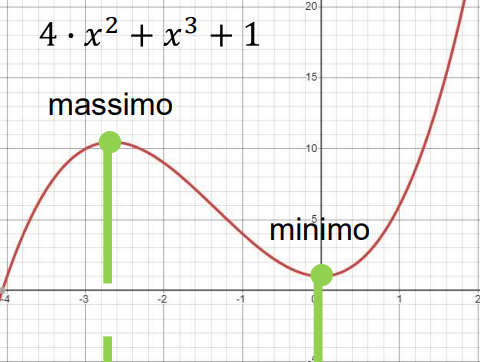
\includegraphics[width = 0.50\textwidth]{Images/1.PNG}
\end{center}
Data una funzione continua $f:[a,b] \rightarrow \mathbb{R}$ e un punto $x_0 \in [a,b]$, si dice che $f$ ha un minimo o massimo locale (o relativo) nel punto 
$x_0$ quando esiste un intorno $l(x_0)$ nel quale risulta
\begin{itemize}
    \item $f(x) \geq f(x_0) \forall x \in l(x_0)$ allora $x_0$ è un \textbf{minimo locale}
    \item $f(x) \leq f(x_0) \forall x \in l(x_0)$ allora $x_0$ è un \textbf{massimo locale}
    \item $x_0$ è un \textbf{minimo locale relativo} se la funzione è decrescente immediatamente a sinistra di $x_0$ e crescente immediatamente a destra
    \item $x_0$ è un \textbf{massimo locale relativo} se la funzione è crescente immediatamente a sinistra di $x_0$ e decrescente immediatamente a destra 
\end{itemize}
Il punto minimo (massimo) locale in cui la funzione $f$ assume il valore minimo (massimo) viene detto \textbf{minimo} (\textbf{massimo}) \textbf{globale} o \textbf{assoluto}.
\subsection{Funzioni in due o più variabili}
Una funzione continua definita come $f: \mathbb{R} \times \mathbb{R} \rightarrow \mathbb{R}$ che associa ad ogni coppia di numeri reali $(x_1, x_2) \in \mathbb{R} \times \mathbb{R} = R^2$ uno
e un solo valore $y \in \mathbb{R}$ viene detta \textbf{funzioni in due variabili} $(x_1, x_2)$, che vengono dette \textbf{variabili indipendenti}, mentre la variabile $y$ viene riferita con il termine di
\textbf{variabile dipendente}.
Questo concetto è generalizzabile al caso in cui si considerino $n$ variabili indipendenti $(x_1, x_2, ..., x_n) \in \mathbb{R}^n$. In questo caso
si parla di funzione $f: \mathbb{R}^n \rightarrow \mathbb{R}$ in $n$ variabili indipendenti, funzione che descrive una "regola" per ottenere dall'insieme delle $n$ variabili indipendenti $(x_1, x_2, ..., x_n)$ un singolo
valore reale di $y$. \newline
Una funzione in $n$ variabili $f: \mathbb{R}^n \rightarrow \mathbb{R}$ viene detta \textbf{funzione lineare} nelle variabili $(x_1, x_2, ..., x_n)$ se è nella forma:
$$f(x_1, x_2, ..., x_n) = a_0 + a_1 \cdot x_1 + a_2 \cdot x_2 + ... + a_n \cdot x_n$$
dove $a_0, a_1, ..., a_n$ sono parametri che assumono valore reale. \newline
Una funzione in $n$ variabili $f: \mathbb{R}^n \rightarrow \mathbb{R}$ viene detta \textbf{funzione quadratica} nelle variabili $(x_1, x_2, ..., x_n)$ se è nella forma:
$$f(x_1, x_2, ..., x_n) = a_0 + \sum_{k=1}^n b_k \cdot x_k + \sum_{i = 1}^n \sum_{j \neq i,1}^n h_{ij} \cdot x_i \cdot x_j + \sum_{k=1}^n h_{kk} \cdot x_k^2$$
\begin{center}
    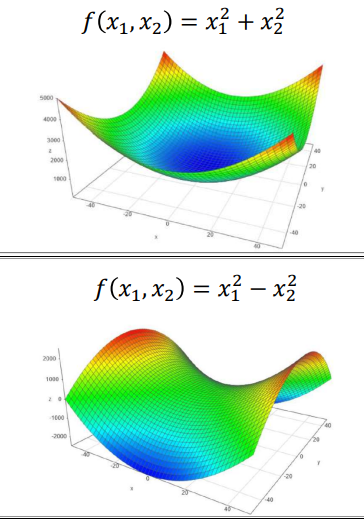
\includegraphics[width = 0.35\textwidth]{Images/2.PNG}
\end{center}
Le \textbf{curve di livello} di una funzione $f: \mathbb{R}^n \rightarrow \mathbb{R}$ sono ottenute disegnando i punti
$(x_1, x_2, ..., x_n)$ in cui la funzione ha valore constante $k$, vale a dire tutti i punti $(x_1, x_2, ..., x_n) \in \mathbb{R}^n$ per i quali vale la seguente uguaglianza
$$f(x_1, x_2, ..., x_n) = k$$
\begin{center}
    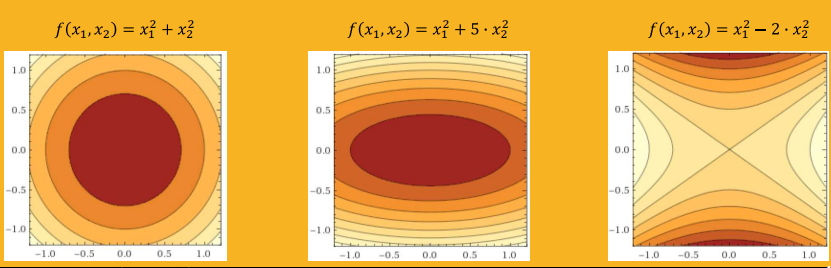
\includegraphics[width = 1\textwidth]{Images/3.PNG}
\end{center}
Dal punto di vista geometrico, le linee di livello sono le \textbf{proiezioni ortogonali} sul piano $Oxy$ delle curve ottenute
intersecando il piano $z=k$ e il grafico della funzione $z = f(x_1, x_2, ..., x_n)$
\begin{center}
    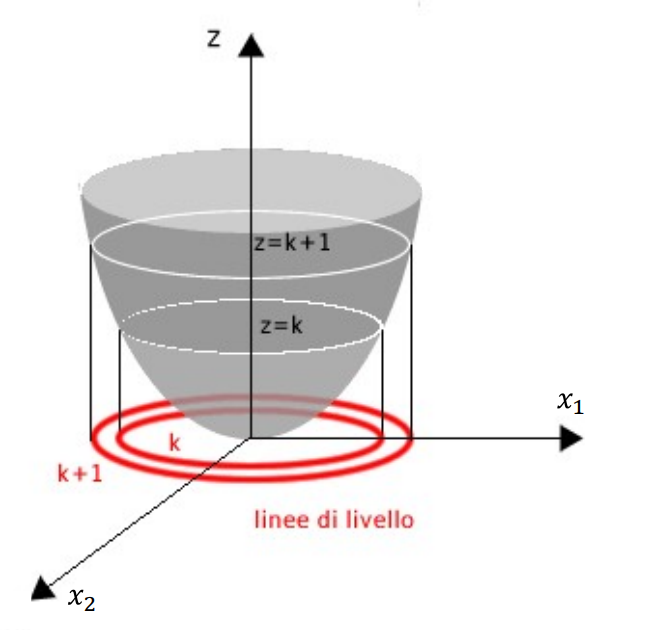
\includegraphics[width = 0.50\textwidth]{Images/4.PNG}
\end{center}
Data la funzione in 2 variabili $f: \mathbb{R}^2 \rightarrow \mathbb{R}$:
\begin{itemize}
    \item Si dice \textbf{derivata parziale rispetto a $x_1$} la seguente funzione:
    $$\frac{\partial f(x_1, x_2)}{\partial x_1} = f_{x_1} = f'_{x_1}$$
    Essa rappresenta il tasso con cui varia la funzione $f(x_1, x_2)$ al variare della variabile $x_1$, quando sia fissato e mantenuto costante
    il valore della variabile $x_2$.
    \item Si dice \textbf{derivata parziale rispetto a $x_2$} la seguente funzione:
    $$\frac{\partial f(x_1, x_2)}{\partial x_2} = f_{x_2} = f'_{x_2}$$
    Essa rappresenta il tasso con cui varia la funzione $f(x_1, x_2)$ al variare della variabile $x_2$, quando sia fissato e mantenuto costante
    il valore della variabile $x_1$
    \item Si dice \textbf{gradiente} il vettore i cui coefficienti sono le derivate parziali della funzione $f(x_1, x_2)$ rispetto alle variabili $x_1$ e $x_2$, esso è denotato nel seguente modo:
    $$\nabla f(x_1, x_2) = \begin{pmatrix}
        \frac{\partial f(x_1, x_2)}{\partial x_1} \\
        \frac{\partial f(x_1, x_2)}{\partial x_2}
    \end{pmatrix} = \begin{pmatrix}
        f'_{x_1} \\
        f'_{x_2}
    \end{pmatrix}$$
\end{itemize}
Data la funzione in 2 variabili $f: \mathbb{R}^2 \rightarrow \mathbb{R}, f(x_1, x_2)$:
\begin{itemize}
    \item Si dice \textbf{derivata parziale seconda rispetto a $x_1$} e $x_1$ la seguente funzione:
    $$\frac{\partial}{\partial x_1} \frac{\partial f(x_1, x_2)}{\partial x_1} = f_{x_1, x_1} = f'_{x_1, x_1}$$
    \item Si dice \textbf{derivata parziale seconda rispetto a $x_1$} e $x_2$ la seguente funzione:
    $$\frac{\partial}{\partial x_1} \frac{\partial f(x_1, x_2)}{\partial x_2} = f_{x_1, x_2} = f'_{x_1, x_2}$$
    \item Si dice \textbf{derivata parziale seconda rispetto a $x_2$} e $x_1$ la seguente funzione:
    $$\frac{\partial}{\partial x_2} \frac{\partial f(x_1, x_2)}{\partial x_1} = f_{x_2, x_1} = f'_{x_2, x_1}$$
    \item Si dice \textbf{derivata parziale seconda rispetto a $x_2$} e $x_2$ la seguente funzione:
    $$\frac{\partial}{\partial x_2} \frac{\partial f(x_1, x_2)}{\partial x_2} = f_{x_2, x_2} = f'_{x_2, x_2}$$
\end{itemize}
In particolare:
$$\frac{\partial}{\partial x_1} \frac{\partial f(x_1, x_2)}{\partial x_2} = f_{x_1, x_2} = f'_{x_1, x_2} = \frac{\partial}{\partial x_2} \frac{\partial f(x_1, x_2)}{\partial x_1} = f_{x_2, x_1} = f'_{x_2, x_1}$$
Data la funzione in 2 variabili $f: \mathbb{R}^2 \rightarrow \mathbb{R}, f(x_1, x_2)$, si dice
\textbf{matrice Hessiana} la matrice quadrata delle derivate parziali:
$$H = \begin{pmatrix}
    f_{x_1, x_1} & f_{x_1, x_2} \\
    f_{x_2, x_1} & f_{x_2, x_2}
\end{pmatrix}$$
\textbf{Condizione necessaria del primo ordine}: Data la funzione in 2 variabili $f: \mathbb{R}^2 \rightarrow \mathbb{R}, f(x_1, x_2)$, un punto
$(x_1, x_2)$ può essere un punto critico (minimo, massimo o sella) solo se il suo gradiente nel punto $(x_1, x_2)$ è nullo:
$$\nabla f(x_1, x_2) = \begin{pmatrix}
    0 \\
    0
\end{pmatrix}$$
Non ne conosciamo però la natura! (Minimo? Massimo? Sella?) \newpage
\textbf{Condizioni sufficienti del secondo ordine}:
Supponiamo che $(x_1, x_2)$ sia un punto critico di $f(x_1, x_2)$. Calcoliamo il determinante della matrice Hessiana:
$$det(H) = f_{x_1,x_1} (x_1, x_2) \cdot f_{x_2 x_2}(x_1, x_2) - (f_{x_1, x_2}(x_1, x_2))^2$$
Abbiamo i seguenti casi:
\begin{itemize}
    \item $det(H) > 0$:
    \begin{itemize}
        \item $f_{x_1, x_1} > 0 \Rightarrow (x_1, x_2)$ è un minimo relativo di $f(x_1, x_2)$
        \item $f_{x_1, x_1} < 0 \Rightarrow (x_1, x_2)$ è un massimo relativo di $f(x_1, x_2)$
    \end{itemize}
    \item $det(H) < 0 \Rightarrow (x_1, x_2)$ è un punto di sella di $f(x_1, x_2)$
\end{itemize}
Data la funzione in 2 variabili $f: \mathbb{R}^2 \rightarrow \mathbb{R}, f(x_1, x_2)$, se la sua matrice Hessiana $H$ è tale per cui
$f_{x_1, x_1} > 0$ e $det(H) > 0$ allora la funzione è \textbf{convessa}. Se la funzione è  convessa, allora ogni punto di minimo e di massimo sono
\textbf{globali} poiché ammette solamente un punto dove il gradiente si annulla
\section{Modelli nella Ricerca Operativa}
Data una funzione
$$f: \mathbb{R}^n \rightarrow \mathbb{R}$$
la chiamiamo \textbf{funzione obbiettivo}.
Un \textbf{problema di ottimizzazione} è formulabile come segue:
\begin{equation*}
    \begin{array}{rrclcl}
    \displaystyle \textrm{opt} & f(x)\\
    \textrm{s.a.} & x \in X & X \subseteq \mathbb{R}^n
    \end{array}
\end{equation*}
$X$ è detta \textbf{regione ammissibile}, cioè l'insieme delle soluzioni $x$ ammissibili dal problema. Inoltre, $\textrm{opt} \in \{\textrm{min}, \textrm{max}\}$. \newline
Se $\textrm{opt} = \textrm{min}$, allora abbiamo un \textbf{problema di minimizzazione}, altrimenti un \textbf{problema di massimizzazione}. \newline
Le variabili che indicano i vincoli ai quali è soggetto il problema sono dette \textbf{variabili decisionali} e identificano una soluzione del problema. \newline
Quindi, un problema di ottimizzazione consiste nel determinare, se esistono, uno o più punti di minimo/massimo $\textbf{x}^*$, assegnazione di valori alle variabili decisionali $\textbf{x}$, della funzione obbiettivo $f$ tra i punti
\textbf{x} che appartengono alla regione ammissibile $X$.
\begin{center}
    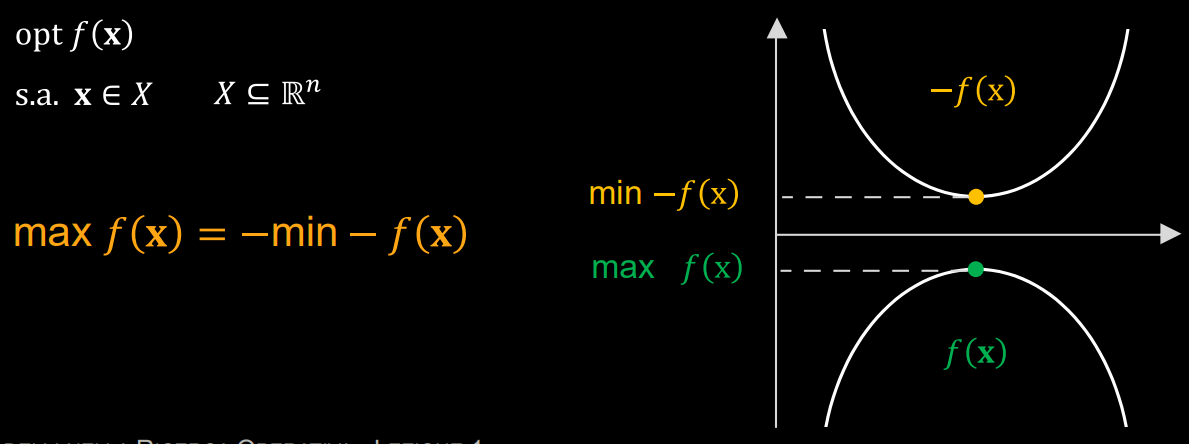
\includegraphics[width = 1\textwidth]{Images/5.PNG}
\end{center}
In particolare, se alcune zone di $\mathbb{R}^n$ non sono ammissibili, si dice che non sono \textbf{eleggibili}. \newline
Quando parliamo di ottimizzazione di una funzione obbiettivo possiamo avere diversi tipi di ottimizzazione: \newline 
\textbf{Ottimizzazione NON vincolata}: la ricerca del/i punto/i di ottimo della funzione obbiettivo viene condotta su tutto lo spazio di definizione
(quindi $X = \mathbb{R}^n)$ della/e variabile/i di decisione \newline
\textbf{Ottimizzazione vincolata}: la ricerca del/i punto/i di ottimo della funzione obbiettivo viene condotta su un sottoinsieme proprio dello spazio di definizione
(cioè $X \subset \mathbb{R}^n)$ della/e variabile/i di decisione
\textbf{Ottimizzazione intera}: le variabili di decisione assumono solo valori interi (quindi $X = \mathbb{Z}^n)$ \newline
\textbf{Ottimizzazione binaria}: Le variabili assumono solo valore 0 e 1 (quindi $X \in \{0,1\}^n$) \newline
\textbf{Ottimizzazione mista}: Alcune variabili assumono valori interi mentre altre variabili assumono solo valori binari. \newline
Se non specificato altrimenti, si deve intendere che \textbf{le variabili decisionali assumono valori reali}.
\subsection{Programmazione matematica}
Quando l'insieme $X$ delle soluzioni ammissibili di un problema di ottimizzazione viene espresso attraverso un sistema di equazione e disequazione, esso prende il nome di problema di
\textbf{programmazione matematica} (PM).
In questo caso un \textbf{vincolo} è un espressione del tipo:
$$g_i(x) \begin{Bmatrix}
    \geq \\
    = \\
    \leq
\end{Bmatrix} 0$$
Con $g_i: X \rightarrow \mathbb{R}$ funzione generica che lega tra loro le variabili decisionali.
In generale, possiamo avere uno o più vincoli. \newline
La \textbf{regione ammissibile} è quindi definita dall'insieme dei vincoli del problema, cioè:
$$X = \left \{x \in \mathbb{R}^n \; con \; g_i(x) \begin{Bmatrix} \leq \\ = \\ \geq \end{Bmatrix}, i = 1,...,m \right \}$$
Osserviamo, quindi, che abbiamo $m$ vincoli ed $n$ variabili. Inoltre
\begin{itemize}
    \item Se $x \in X$ allora $x$ è soluzione \textbf{ammissibile}
    \item Se $x \not\in X$ allora $x$ \textbf{non è una soluzione ammissibile} (soluzione inammissibile)
\end{itemize}
In un problema di ottimizzazione, abbiamo le seguenti possibilità riguardo la regione ammissibile:
\begin{itemize}
    \item \textbf{Problema non ammissibile}: $X = \emptyset$ (regione ammissibile vuota, nessuna soluzione ammissibile, problema mal posto)
    \item \textbf{Problema illimitato}, cioè:
    \begin{itemize}
        \item $\forall c \in \mathbb{R}, \exists x_c \in X | f(x_c) \leq c$ se $\textrm{opt} = \textrm{min}$ (illimitato inferiormente)
        \item $\forall c \in \mathbb{R}, \exists x_c \in X | f(x_c) \geq c$ se $\textrm{opt} = \textrm{max}$ (illimitato superiormente)
    \end{itemize}
    \item \textbf{Problema con soluzione ottima unica}
    \item \textbf{Problema con più di una soluzione ottima} (anche \textbf{infinite}): tutte le soluzione ottime hanno egual valore della funzione obbiettivo
\end{itemize}
\begin{center}
    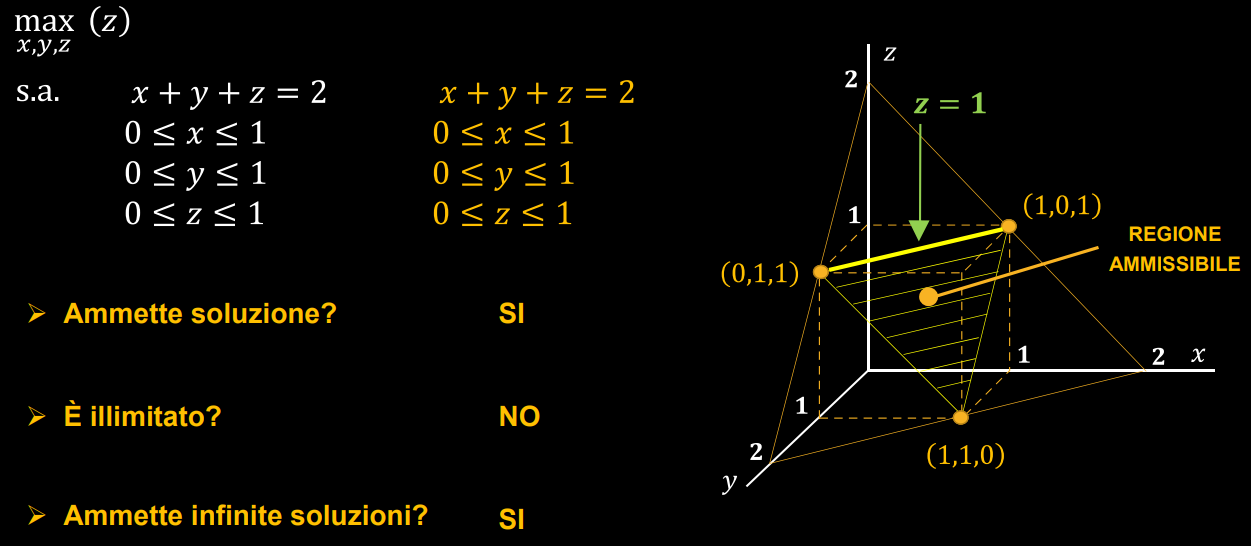
\includegraphics[width = 0.90\textwidth]{Images/6.PNG}
\end{center}
\subsection{Ottimi globali e ottimi locali}
La risoluzione di un problema di programmazione matematica consiste nel trovare una soluzione ammissibile che sia un \textbf{ottimo globale},
vale a dire un vettore $\textbf{x}^* \in X$ tale che:
\begin{itemize}
    \item $f(\textbf{x}^*) \leq f(x) \forall x \in X$ se $\textrm{opt} = \textrm{min}$
    \item $f(\textbf{x}^*) \geq f(x) \forall x \in X$ se $\textrm{opt} = \textrm{max}$
\end{itemize}
\begin{Osservazione}
    Un problema di ottimizzazione può avere:
    \begin{itemize}
        \item Più di un ottimo locale
        \item Più di un ottimo globale
    \end{itemize}
\end{Osservazione}
\begin{Osservazione}
    Un punto di ottimo globale è anche di ottimo locale
\end{Osservazione}
\begin{Osservazione}
    Nel caso di una funzione obbiettivo \textbf{convessa}, vi è un unico ottimo globale
\end{Osservazione}
Anche qui abbiamo diversi casi possibili:
\begin{itemize}
    \item \textbf{Programmazione lineare}: in questo caso ci troviamo davanti ad un problema con questa formulazione:
    $$\textrm{opt} \; f(x) = \textbf{c}^T \textbf{x} \; (lineare)$$
    La regione ammissibile è quindi formulabile in questo modo:
    $$X = \left \{x \in \mathbb{R}^n \bigg | g_i(x) \begin{Bmatrix} \leq \\ = \\ \geq \end{Bmatrix}, i = 1,...,m \right \}$$
    con $g_i(x) = \textbf{a}_j^T\textbf{x} - b_i$ vincoli \textbf{lineari}
    \item \textbf{Programmazione Lineare Intera}: in questo caso ci troviamo davanti ad un problema con questa formulazione:
    $$\textrm{opt} \; f(x) = \textbf{c}^T \textbf{x} \; (lineare)$$
    La regione ammissibile è quindi formulabile in questo modo:
    $$X = \left \{x \in \mathbb{Z}^n \bigg | g_i(x) \begin{Bmatrix} \leq \\ = \\ \geq \end{Bmatrix}, i = 1,...,m \right \}$$
    con $g_i(x) = \textbf{a}_j^T\textbf{x} - b_i$ vincoli \textbf{lineari}
    \item \textbf{Programmazione non lineare}: in questo caso ci troviamo davanti ad un problema con questa formulazione:
    $$\textrm{opt} \; f(x) \; (lineare \; o \; non \; lineare)$$
    La regione ammissibile è quindi formulabile in questo modo:
    $$X = \left \{x \in \mathbb{R}^n \bigg | g_i(x) \begin{Bmatrix} \leq \\ = \\ \geq \end{Bmatrix}, i = 1,...,m \right \}$$
    con $g_i(\textbf{x})$ vincoli \textbf{lineari} o \textbf{non lineari}. È importante notare come, in questo caso, almeno un vincolo o
    la funzione obbiettivo sono NON lineari
\end{itemize}
\section{Programmazione lineare}
La programmazione lineare (PL) è quella branca della ricerca operativa che si occupa di studiare algoritmi di risoluzione per problemi di ottimizzazione lineari.
Un problema di programmazione lineare è strutturato come segue:
$$\underset{\textbf{x} \in X}{\textrm{opt}}Z = \sum_{j=1}^{n} c_j \cdot x_j \; (Funzione \; obbiettivo \; Z \; con \; n, \; numero \; di \; variabili \; decisionali)$$
$$\sum_{j=1}^n a_{ij} \cdot x_j \leq b_i, i = 1,...,m \; (Vincoli: \; regione \; ammissibile \; X \; con \; m, numero \; di \; vincoli)$$
Con: \newline
$x_j$ \textbf{variabili decisionali} \newline
$\left. \begin{matrix}
        c_j \; \textbf{coefficienti di costo} \\
        a_{ij}\; \textbf{termini noti sinistri} \\
        b_i \; \textbf{termini noti destri} \\
\end{matrix}\right\}$ Parametri \newline
Un problema di programmazione lineare si poggia sulle seguenti \textbf{assunzioni implicite}:
\begin{itemize}
    \item \textbf{Proporzionalità}: il contributo di ogni variabile decisionale, al valore della funzione obbiettivo, è proporzionale rispetto al valore assunto dalla variabile stessa
    \item \textbf{Additività}: ogni funzione è la somma dei contributi delle variabili decisionali
    \item \textbf{Continuità}: qualunque valore delle variabili decisionali in $\mathbb{R}^n$ è accettabile
    \item \textbf{Certezza}: il valore assegnato ad ogni parametro è assunto essere noto o costante 
\end{itemize}
Vediamole nel dettaglio:
\subsection{Assunzione di Proporzionalità}
Il contributo di ogni attività al valore della \textbf{funzione obbiettivo} $Z$ è proporzionale al \textbf{livello dell'attività} $x_j$ secondo:
$$Z = \sum_{j=1}^n c_j \cdot x_j$$
Analogamente, il contributo di ogni attività al \textbf{vincolo "i"} è proporzionale al \textbf{livello di attività} $x_j$ secondo
$$\sum_{j=1}^n a_{ij} \cdot x_j \leq b_i$$
Vediamo un esempio:
\begin{center}
    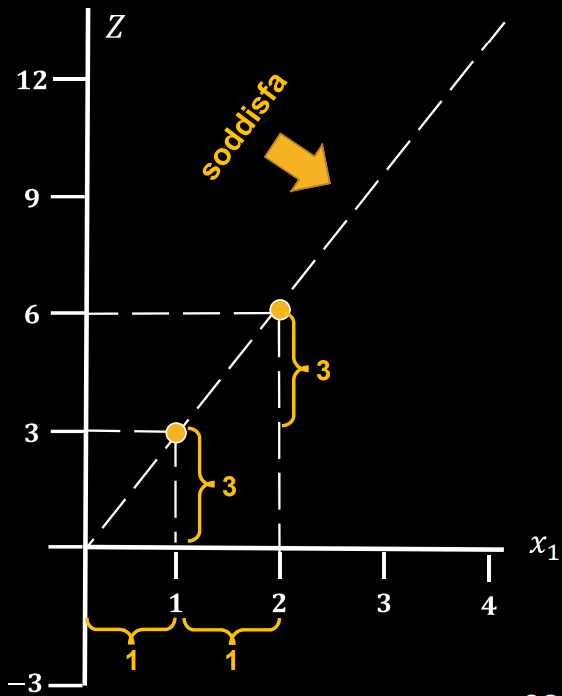
\includegraphics[width = 0.40\textwidth]{Images/7.PNG}
\end{center}
\begin{center}
    
\includegraphics[width = 0.45\textwidth]{Images/8.PNG}
\end{center}
\subsection{Assunzione di additività}
In un problema di programmazione lineare, il valore assunto da ogni funzione, sia essa \textbf{funzione obbiettivo} o vincolo, è dato dalla somma dei contributi individuali delle rispettive attività.
Vediamo un esempio:
\begin{center}
    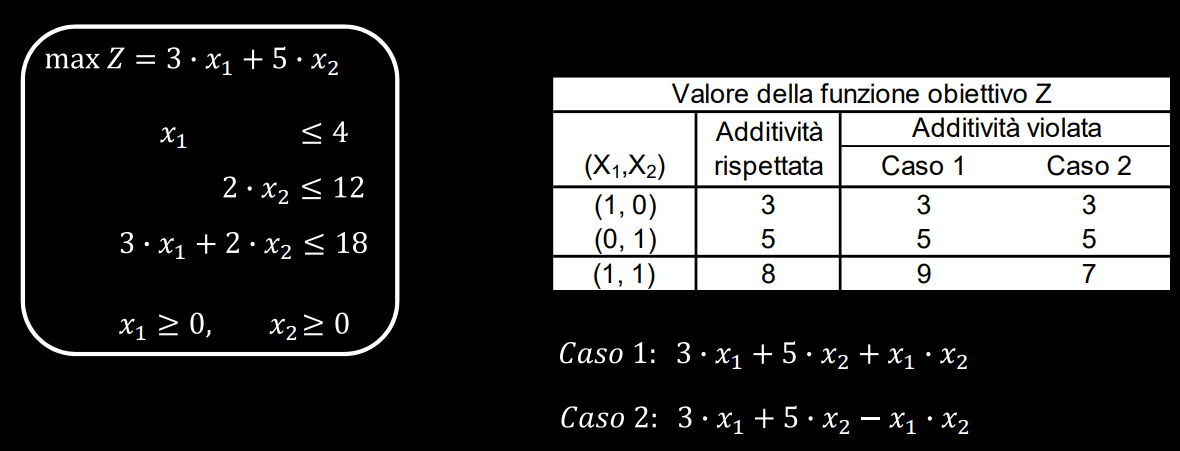
\includegraphics[width = 0.95\textwidth]{Images/9.PNG}
\end{center}
\subsection{Assunzione di continuità}
Le variabili decisionali in un problema di programmazione lineare (PL) sono libere di assumere qualsiasi valore, inclusi valori non interi che soddisfino i vincoli funzionali ed i vincoli di non negatività.
In altri termini le variabili decisionali sono continue.
In alcune condizioni può accadere che le variabili decisionali non possano che assumere valori interi; in questi casi si parla di problema di programmazione lineare intera o a numeri interi.
\subsection{Assunzione di certezza}
Il valore assegnato ad ogni parametro di un problema di programmazione lineare è assunto essere noto con certezza e costante.
\subsection{Soluzione grafica ad un problema di programmazione lineare}
Per risolvere i problemi di programmazione lineare, possiamo adottare una \textbf{procedura grafica}, determinando i valori delle variabili decisionali
$x_1, x_2$ che rispettano i vincoli, ed al tempo stesso rendono massimo il valore $Z$ della funzione obbiettivo.
La \textbf{soluzione grafica} si compone di:
\begin{itemize}
    \item Disegno della regione ammissibile
    \item Determinazione dell'ottimo
\end{itemize}
\subsubsection{Vincolo di uguaglianza}
I vincoli $g_i(\textbf{x})$ possono essere:
\begin{itemize}
    \item \textbf{Rette}: $g_i(x) = 0$
    \item \textbf{Semipiani}: $g_i(x) \leq 0$
\end{itemize}
Un vincolo del tipo $a_1 \cdot x_1 + a_2 \cdot x_2 = b$ è una \textbf{retta nel piano}.
La retta è perpendicolare al vettore $\nu = (a_1, a_2)$. Abbiamo quindi i seguenti casi:
\begin{center}
    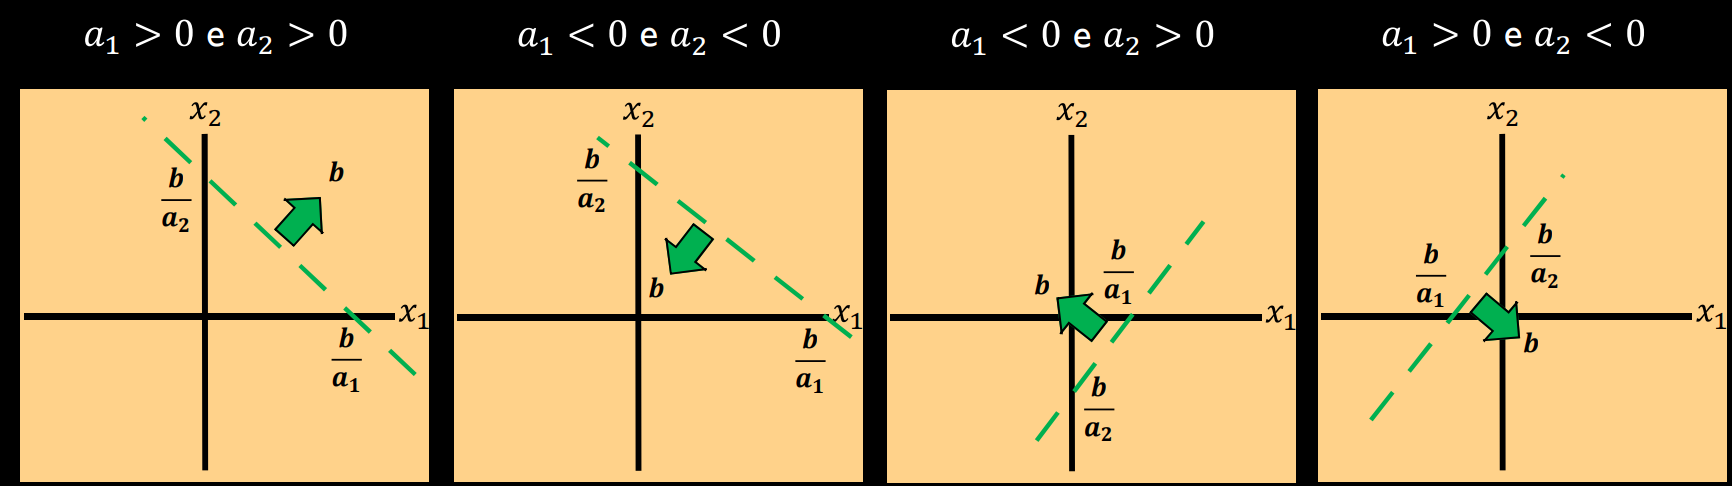
\includegraphics[width = 1\textwidth]{Images/10.PNG}
\end{center}
Come rappresentiamo però un semipiano?
\begin{enumerate}
    \item Disegniamo la retta associata $(a_1 \cdot x_1 + a_2 \cdot x_2 \leq b)$
    \item Scegliamo un punto non appartenente a tale retta (torna comodo 0)
    \begin{itemize}
        \item Se il punto verifica la disuguaglianza allora scegliamo il semipiano che lo contiene
        \item Altrimenti scegliamo l'altro semipiano
    \end{itemize}
\end{enumerate}
\begin{center}
    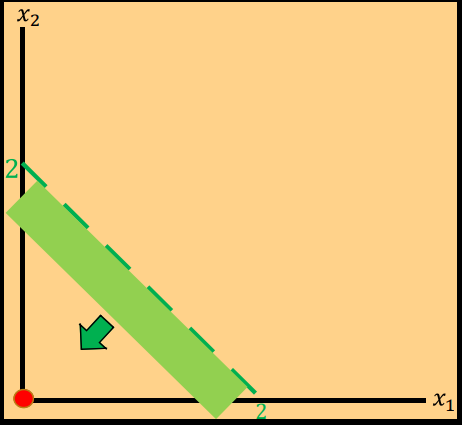
\includegraphics[width = 0.30\textwidth]{Images/11.PNG}
\end{center}
\subsubsection{Vincoli funzionali di $\leq$}
In maniera generalizzata, possiamo pensare che un problema di programmazione lineare è formulato in questo modo:
\begin{equation*}
    \begin{array}{ll}
    \displaystyle \textrm{opt} & \; Z = c_1 \cdot x_1 + c_2 \cdot x_2 +...+ c_n \cdot x_n\\
    \textrm{s.a.} & a_{11} \cdot x_1 + a_{12} \cdot x_2 +...+ a_{1n} \cdot x_n \leq b_1 \\
    \phantom{} & a_{21} \cdot x_1 + a_{22} \cdot x_2 +...+ a_{2n} \cdot x_n \leq b_2 \\
    \phantom{} &... ... ... + ... ... ... + ... + ... ... ... \leq ... \\
    \phantom{} & a_{m1} \cdot x_1 + a_{m2} \cdot x_2 +...+ a_{mn} \cdot x_n \leq b_m \\
    \phantom{} &x_1 \geq 0, x_2 \geq 0, x_3 \geq 0 ..., x_m \geq 0
    \end{array}
\end{equation*}
Con
\begin{itemize}
    \item $Z$ funzione obbiettivo
    \item $\left. \begin{matrix*}[l]
    a_{11} \cdot x_1 + a_{12} \cdot x_2 +...+ a_{1n} \cdot x_n \leq b_1 \\
    a_{21} \cdot x_1 + a_{22} \cdot x_2 +...+ a_{2n} \cdot x_n \leq b_2 \\
    ... ... ... + ... ... ... + ... + ... ... ... \leq ... \\
    a_{m1} \cdot x_1 + a_{m2} \cdot x_2 +...+ a_{mn} \cdot x_n \leq b_m \\
    \end{matrix*}\right\}$ Vincoli funzionali
    \item $x_1 \geq 0, x_2 \geq 0, x_3 \geq 0 ..., x_m \geq 0$ vincoli di non negatività
\end{itemize}
In particolare quindi:
\begin{itemize}
    \item $Z =$ valore della misura di prestazione
    \item $x_j =$ livello dell'attività j
    \item $c_j =$ incremento del valore della misura di prestazione $Z$ corrispondente all'incremento di un'unità del valore dell'attività $x_j$
    \item $b_i =$ quantità di risorsa "$i$" allocabile alle attività $x_j, j = 1,..,n$
    \item $a_{ij} =$ quantità di risorsa "$i$" consumata da ogni unità di attività $x_j, j=1,...,n$
\end{itemize}
\subsubsection{Vincoli funzionali di $\geq$ e =}
Generalizzando al caso con \textbf{$n$ variabili decisionali} ed \textbf{$m$ vincoli}, otteniamo la seguente formulazione di un \textbf{problema di programmazione lineare}: \newline
\textbf{Funzione obbiettivo}: $\textrm{opt}\; Z$ \newline
\textbf{Vincoli}:
\begin{equation*}
    \begin{array}{ll}
        a_{11} \cdot x_1 + a_{12} \cdot x_2 + ... + a_{1n} \cdot x_n \leq b_1 \\
        a_{21} \cdot x_1 + a_{22} \cdot x_2 + ... + a_{2n} \cdot x_n \geq b_2 \\
        ... \\
        a_{n1} \cdot x_1 + a_{n2} \cdot x_2 + ... + a_{nm} \cdot x_n \leq b_n \\
    \end{array}
\end{equation*}
In questo caso quindi, siamo nel caso per il quale \textbf{$x_2$ non è vincolata} da nessun valore.
Inoltre, ogni vincolo di $\geq$ e $=$ può essere riscritto nella seguente forma:
\begin{itemize}
    \item $g_i(x) \geq b_i \rightarrow -g_i(x) \leq b_i$
    \item $g_i(x) = b_i \rightarrow \begin{cases}
        g_i(x) \geq b_i \\
        g_i(x) \leq b_i
    \end{cases}$
\end{itemize}
\subsubsection{Regione ammissibile}
La regione ammissibile $X$ è data dal soddisfacimento dei vari vincoli (Rette e semipiani):
$$X = \left \{\textbf{x} \in \mathbb{R}^n \middle | g_i(x) = \begin{Bmatrix}
    \geq \\
    = \\
    \leq
\end{Bmatrix}0, i=1,...,m \right \} \; con \; g_i(x) = \textbf{a}_i^T \textbf{x} - b_i$$ 
dove $\textbf{a} \in \mathbb{R}^n, \textbf{b} \in \mathbb{R}^m$ \newline
La regione ammissibile, da un punto di vista geometrico, corrisponde ad un \textbf{poliedro convesso in $\mathbb{R}^n$}.
La regione ammissibile può essere \textbf{limitata} (\textbf{politopo}) o illimitata
\begin{center}
    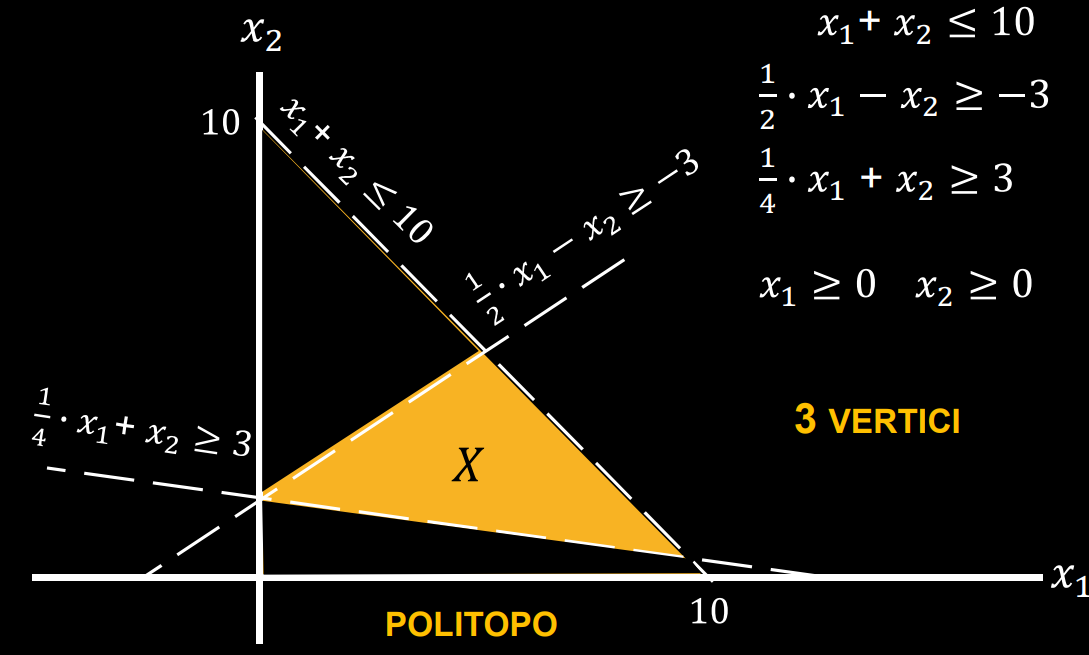
\includegraphics[width = 0.65\textwidth]{Images/12.PNG}
\end{center}
Si possono verificare quattro soluzioni:
\begin{itemize}
    \item Il problema di programmazione lineare \textbf{ammette una sola soluzione ottima} in un \textbf{vertice del poligono convesso}
    che delimita la regione ammissibile.
    \item Il problema di programmazione lineare \textbf{ammette infinite soluzioni ottime} in un \textbf{lato del poligono convesso} che delimita la regione ammissibile
    se la direzione di decrescita è perpendicolare ad un lato del poligono
    \item Il problema di programmazione lineare \textbf{ammette infinite soluzioni} perché la regione ammissibile è illimitata e la funzione obbiettivo è illimitata superiormente (se è di massimizzazione)
    o inferiormente (se di minimizzazione)
    \item Il problema di programmazione lineare \textbf{non ammette soluzione} perché la regione ammissibile è vuota
\end{itemize}
Per risolvere quindi un problema di programmazione lineare graficamente dobbiamo quindi:
\begin{enumerate}
    \item Disegnare la regione ammissibile
    \item Cercare di massimizzare (minimizzare) la soluzione, riportando ciò che troviamo sul grafico
\end{enumerate}
In particolare, per problemi in due variabili $x_1$ e $x_2$, il punto due può essere visto come segue:
\begin{center}
    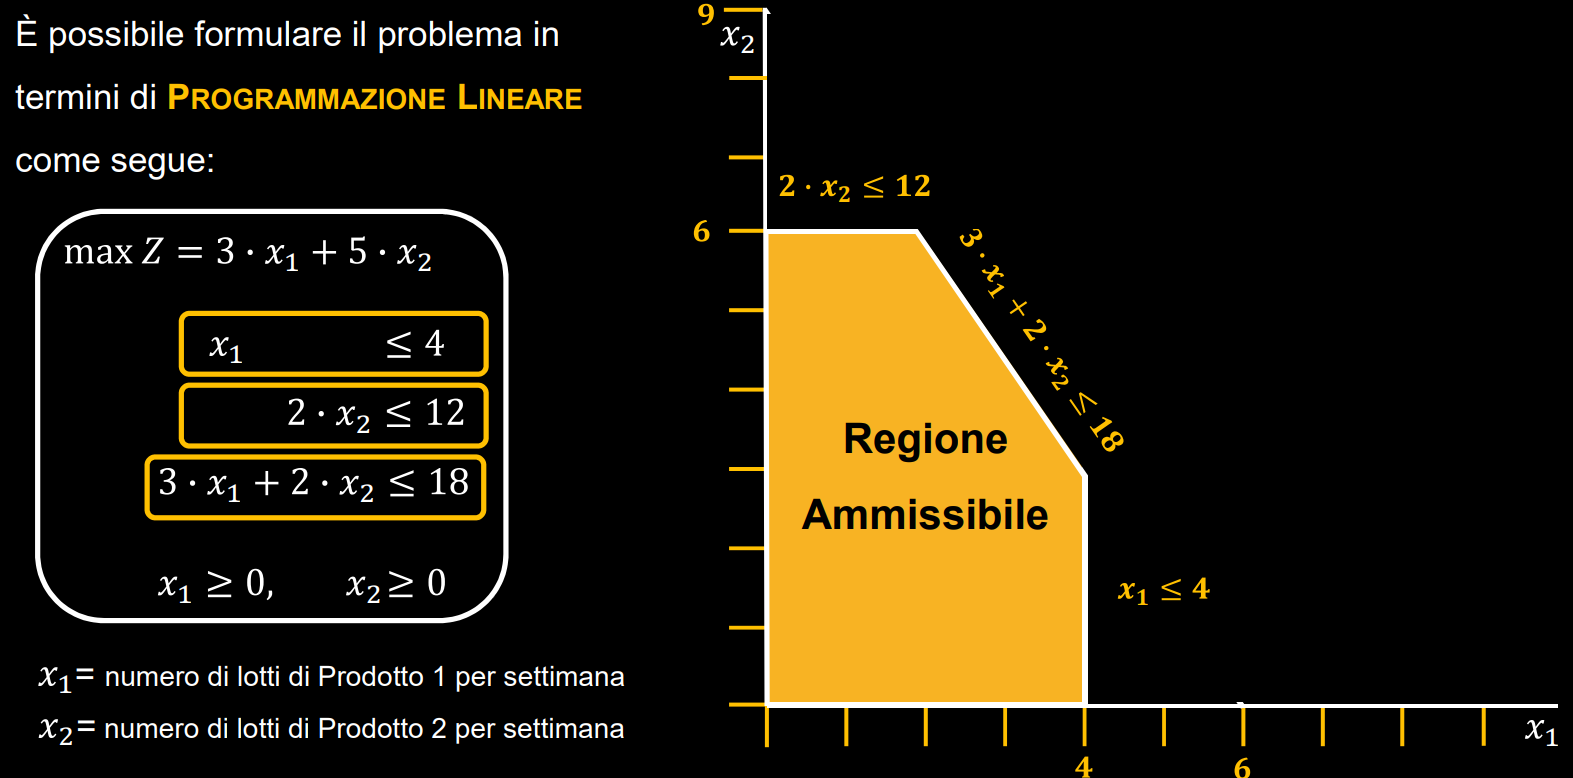
\includegraphics[width = 0.85\textwidth]{Images/13.png}
\end{center}
Riportiamo la regione ammissibile nel piano 3D e troviamo dei valori per $x_1, x_2$ che diano lo stesso valore
una volta sostituiti nella funzione obbiettivo (nell'immagine, abbiamo che i valori $x_1 = 0, x_2 = 5$ e $x_1 = 3, x_2 = 0$)
\begin{center}
    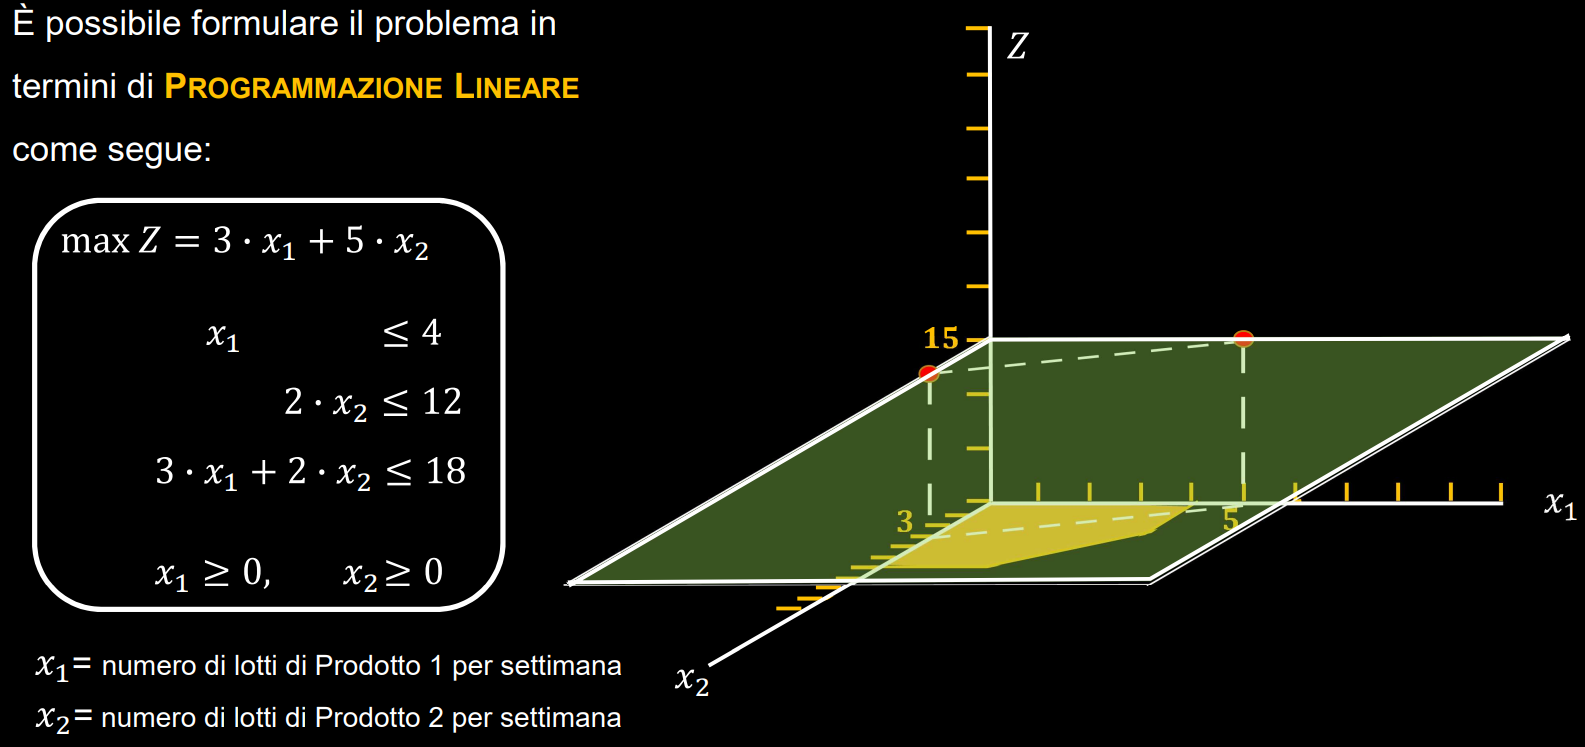
\includegraphics[width = 0.95\textwidth]{Images/14.png}
\end{center}
Continuando così, usiamo il piano creato dalla funzione obbiettivo nello spazio 3D per capire se stiamo uscendo dalla regione ammissibile o meno:
\begin{center}
    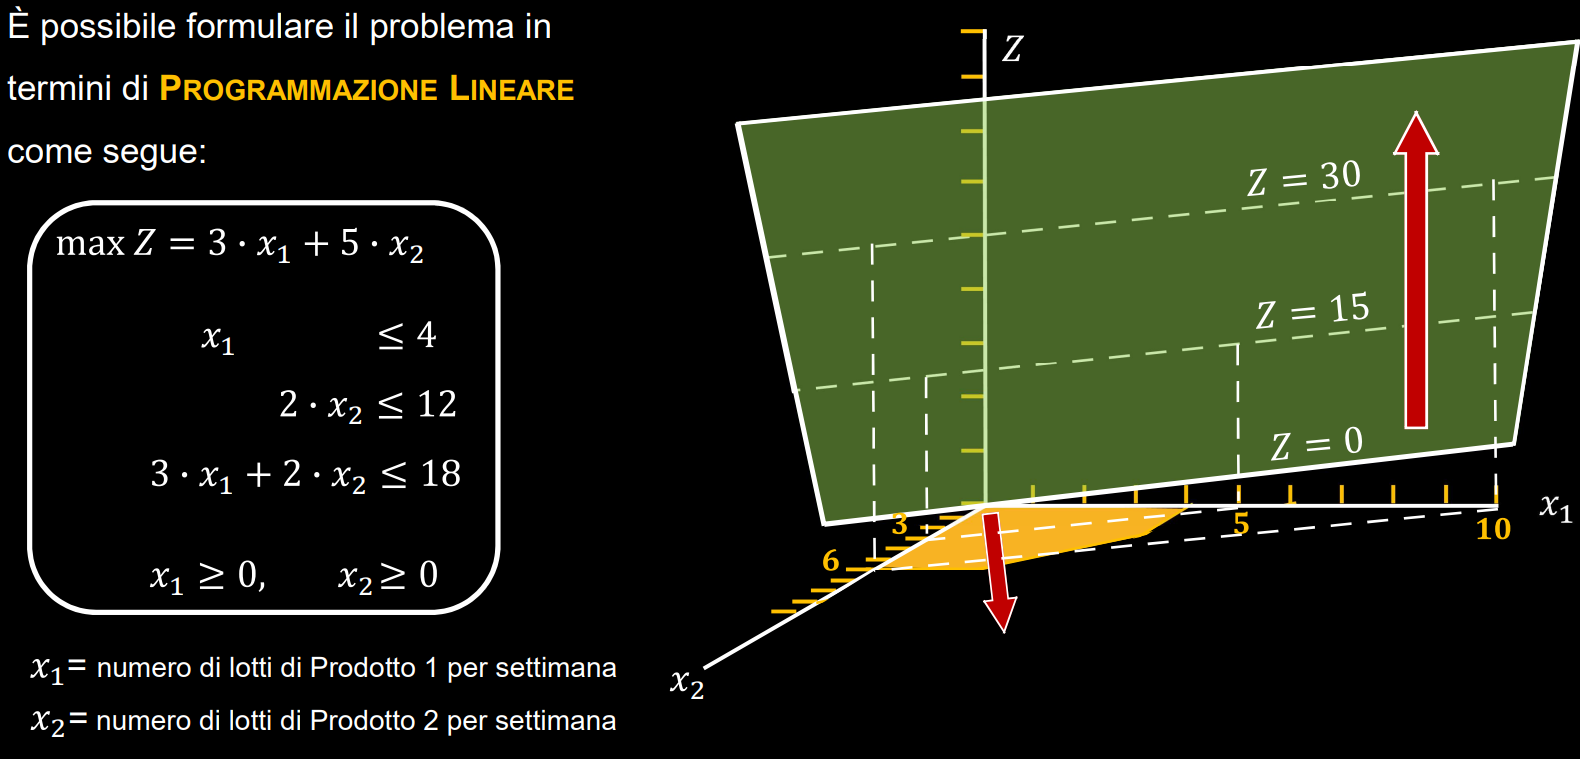
\includegraphics[width = 0.90\textwidth]{Images/15.png}
\end{center}
\begin{center}
    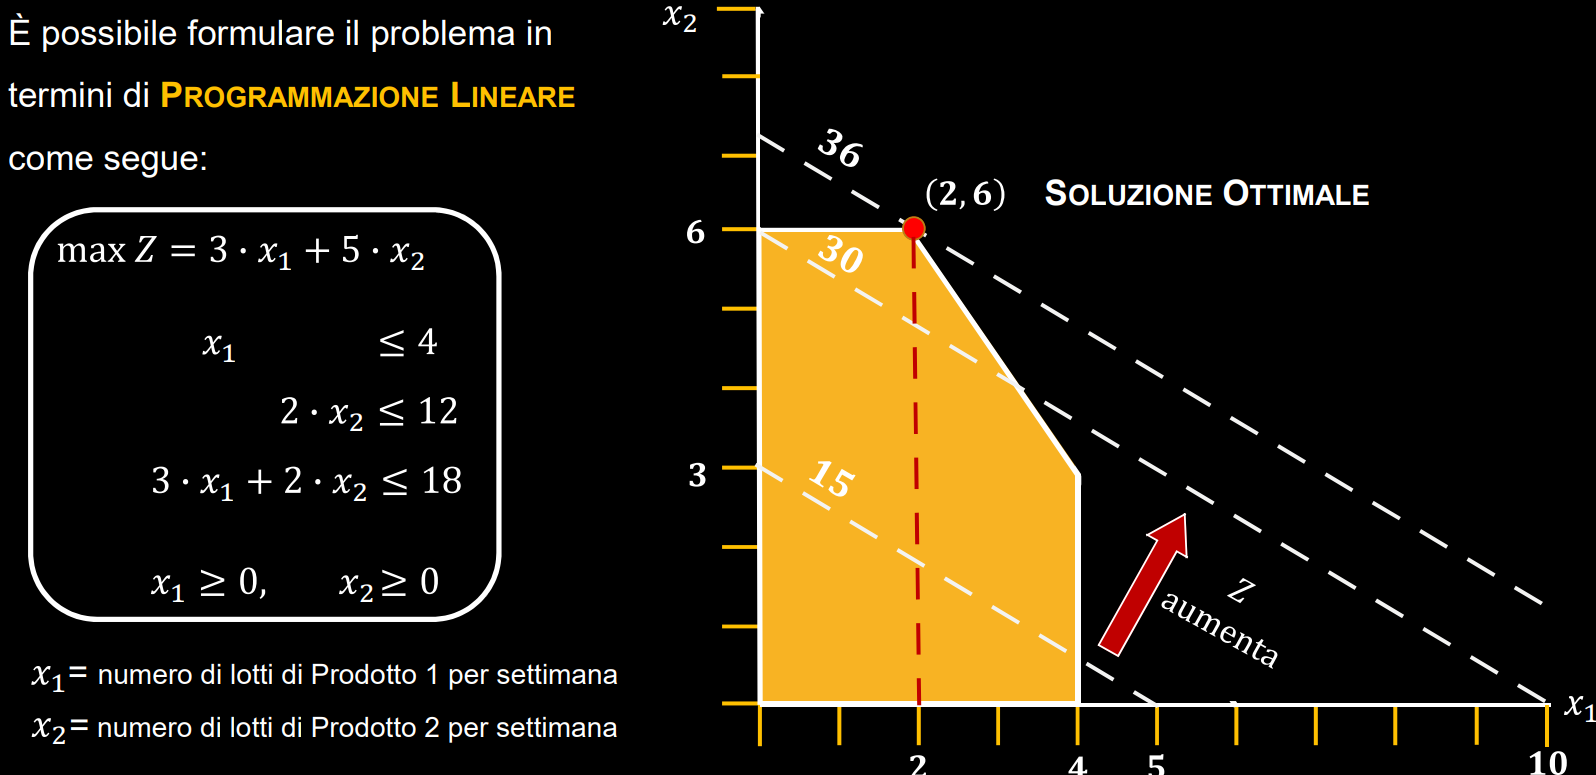
\includegraphics[width = 0.90\textwidth]{Images/16.png}
\end{center}
\subsection{Minimum cost flow problem}
Supponiamo di trovarci in questa situazione:
l'azienda \textbf{distribution unlimited} produrrà un nuovo prodotto in \textbf{due fabbriche differenti},
successivamente i prodotti verranno inviati a \textbf{due magazzini}, ogni fabbrica potrà spedire i propri prodotti ai due magazzini.
La rete distributiva è mostrata di seguito:
\begin{center}
    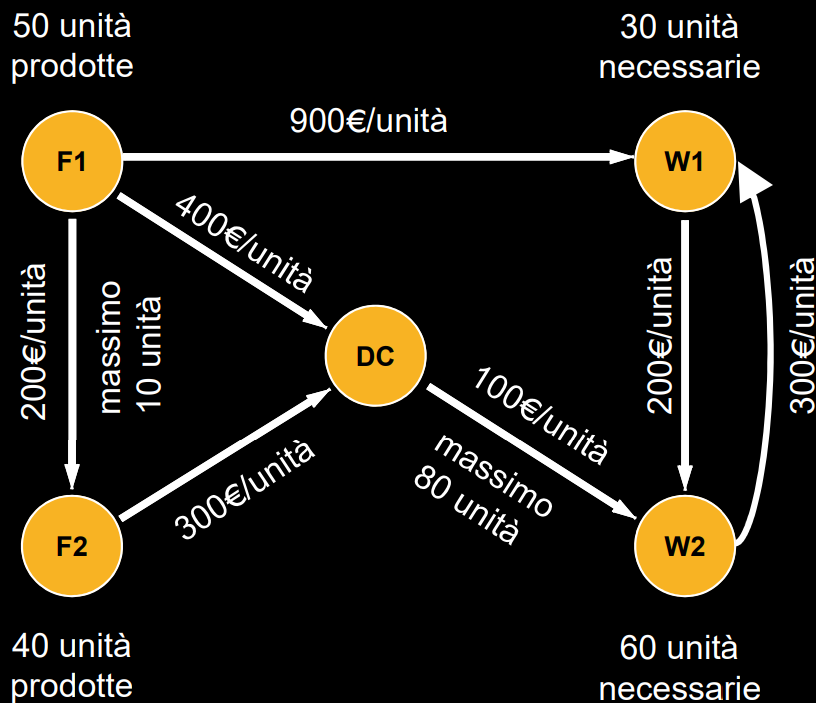
\includegraphics[width = 0.55\textwidth]{Images/17.png}
\end{center}
Il problema consiste nel determinare quante unità di prodotto spedire dalle due fabbriche \textbf{$F1$} e \textbf{$F2$} ai due magazzini
\textbf{$W1$} e \textbf{$W2$}, utilizzando anche il centro di distribuzione \textbf{$DC$}, con l'obbiettivo di \textbf{minimizzare i costi di spedizione}. \newline
Questo tipi di problema prendono il nome di \textbf{Minimum cost flow problems}. Risolviamo l'esempio come segue: \newline
Sette corsie di spedizione richiedono sette variabili decisionali:
$$x_{F1 \rightarrow F2}, x_{F1 \rightarrow W1}, x_{F1 \rightarrow DC}$$
$$x_{F2  \rightarrow DC}$$
$$x_{DC \rightarrow W2}$$
$$x_{W1 \rightarrow W2}$$
$$x_{W2 \rightarrow W1}$$
Troviamo i seguenti vincoli:
\begin{itemize}
    \item \textbf{Vincoli di non negatività}:
    \begin{equation*}
        \begin{array}{ll}
            x_{F1 \rightarrow F2}, x_{F1 \rightarrow W1}, x_{F1 \rightarrow DC} \geq 0 \\
            x_{F2  \rightarrow DC} \geq 0 \\
            x_{DC \rightarrow W2} \geq 0 \\
            x_{W1 \rightarrow W2} \geq 0  \\
            x_{W2 \rightarrow W1} \geq 0
        \end{array}
    \end{equation*}
    \item \textbf{Vincoli di capacità massima}
    \begin{equation*}
        \begin{array}{ll}
            x_{F1 \rightarrow F2} \leq 10 \\
            x_{DC \rightarrow W2} \leq 80
        \end{array}
    \end{equation*}
    \item \textbf{Vincoli di conservazione del flusso}: $outflow - inflow = unita' necessarie$ \newline
    Questo vincolo in sostanza impone che \textbf{la somma dei flussi entranti in ogni nodo deve essere pari al flusso in uscita dal nodo medesimo}
\end{itemize}
IL problema che desideriamo risolvere consiste nel determinare \textbf{quante unità di prodotto} spedire dalle due fabbriche $F1$ e $F2$ ai due magazzini
$W1$ e $W2$, utilizzando anche il \textbf{centro di distribuzione DC}, con l'obbiettivo di minimizzare il costo di spedizione. Il \textbf{costo di spedizione per unità di prodotto}
è indicato per ogni arco di spedizione.
La funzione obbiettivo è:
$$\min Z = 2 \cdot x_{F1 \rightarrow F2} + 4 \cdot x_{F1 \rightarrow DC} + 9 \cdot x_{F1 \rightarrow W1} + 3 \cdot x_{F2 \rightarrow DC} + x_{DC \rightarrow W2} + 3 \cdot x_{W1 \rightarrow W2} + 2 \cdot x_{W2 \rightarrow W1}$$
Una volta calcolati i vincoli visti sopra, possiamo risolvere il problema di programmazione lineare.
\subsection{Metodo del simplesso}
Il metodo del simplesso è un algoritmo per la risoluzione dei problemi di programmazione lineare.
Nel caso medio, il tempo computazionale dell'algoritmo è \textbf{lineare rispetto al numero di variabili}.
Nel caso peggiore, invece, può risultare \textbf{esponenziale}.
Esso è una procedura algebrica, tuttavia i suoi concetti base hanno radici geometriche.
Consideriamo la seguente regione ammissibile:
\begin{center}
    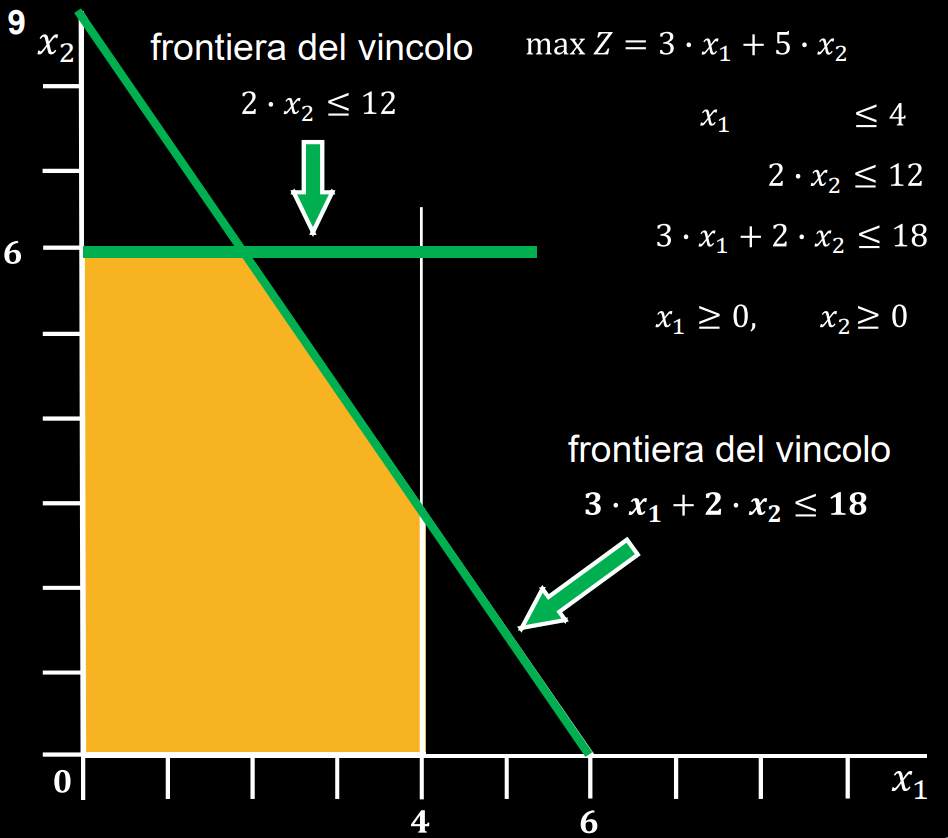
\includegraphics[width = 0.55\textwidth]{Images/18.png}
\end{center}
I \textbf{vertici} si trovano all'intersezione di coppie di frontiere di vincoli.
Per ogni problema di programmazione lineare con $n$ variabili decisionali, due vertici (soluzioni vertici)
si dicono \textbf{adiacenti} se condividono $n-1$ frontiere di vincoli.
Due vertici adiacenti sono collegati da un segmento che giace sull'intersezione delle frontiere dei vincoli condivisi.
Questo segmento viene detto \textbf{spigolo} della regione ammissibile.
\textbf{Non tutti i vertici tuttavia sono soluzioni del problema di programmazione lineare}; lo sono solamente quelli che giacciono sulla regione ammissibile.
L'interesse per i vertici adiacenti sta nella seguente proprietà di cui godono: \newline
\textbf{Test di ottimalità}: Si consideri ogni problema di programmazione lineare tale da ammettere almeno una soluzione ottimale.
Se una soluzione vertice \textbf{non ammette} soluzioni vertice a lei adiacenti con valore della funzione obbiettivo $Z$ migliore, allora la soluzione in questione è \textbf{ottimale}.
Come già detto, il metodo del simplesso è un \textbf{algoritmo} e quindi è formato da una serie di passi:
\begin{enumerate}
    \item 
\end{enumerate}












\end{document}
